\section{Estruturando a Aplicação}
%---------------------------------------------------------------------[ Início ]
\begin{frame}[fragile,t]{Criando Um Help}
    \begin{itemize}
      \item  Um helper será criado para promover o reúso e evitar a repetição 
        de código em uma aplicação. 
    \end{itemize}
    \begin{exampleblock}{\tiny\textbf{caminho: }\url{app/helpers/application_helper.rb}}
      \lstinputlisting[style=RubyInputStyle, basicstyle=\tiny\ttfamily, firstline=1, lastline=10]{rails/codigos/microblog_4/app/helpers/application_helper.rb}
  \end{exampleblock}
\end{frame} 
%---------------------------------------------------------------------[ Início ]
\begin{frame}[fragile,t]{Estruturando a Aplicação}
    \begin{itemize}
      \item  Uma aplicação web deve ser estruturada de forma a facilitar o seu uso.
        Uma ferramentas utilizadas para isso é o protótipo essencial. A ideia inicial
        para a aplicação Microblog foi pensada. 
      \begin{figure}[h!]
        \centering
        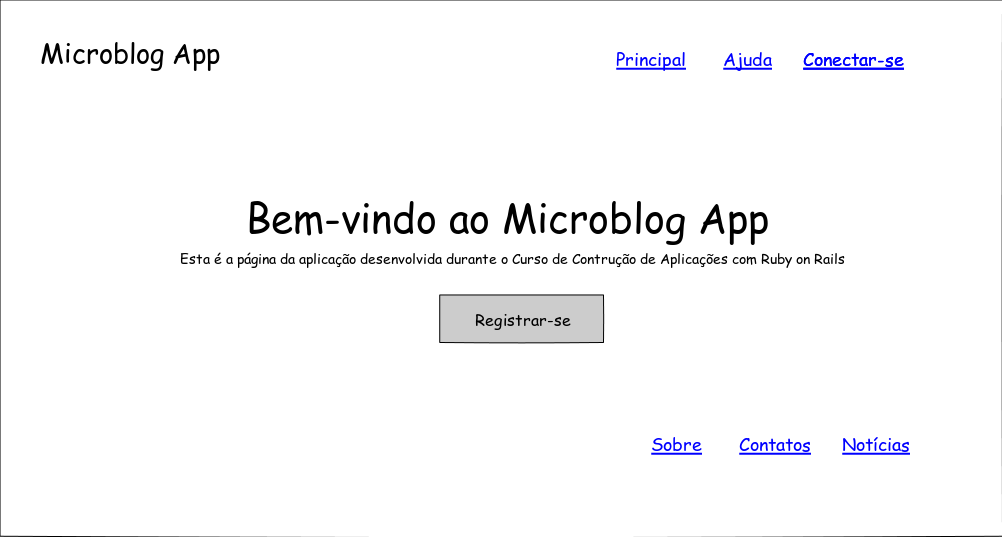
\includegraphics[width=0.85\textwidth]{rails/imagens/esboco-da-pagina-princiapl.png}
      \end{figure}
    \end{itemize}
\end{frame} 
%---------------------------------------------------------------------[ Início ]
\begin{frame}[allowframebreaks, fragile,t]{Navegação da Aplicação}
  \begin{exampleblock}{\tiny\textbf{caminho: }\url{app/views/layouts/application.html.erb}}
      \lstinputlisting[style=RubyInputStyle, basicstyle=\tiny\ttfamily, firstline=8, lastline=28]{rails/codigos/microblog_4/app/views/layouts/application.html.erb}
  \end{exampleblock}
  \framebreak
  \begin{exampleblock}{\tiny\textbf{caminho: }\url{app/views/layouts/application.html.erb}}
      \lstinputlisting[style=RubyInputStyle, basicstyle=\tiny\ttfamily, firstline=1, lastline=15]{rails/codigos/microblog_4/app/views/paginas_estaticas/principal.html.erb}
  \end{exampleblock}
\end{frame} 

